\clearpage
\makeatletter
\efloat@restorefloats
\makeatother


\begin{appendix}
\hypertarget{section}{%
\section{}\label{section}}

Additional analyses were conducted to clarify the effect of task on
classification accuracy. These supplementary analyses were not seen as
central to the current study, but could prove to be informative to
researchers attempting to replicate or extend these findings in the
future. The results from the primary analyses showed that classification
accuracies were the lowest for the Memorize condition, but these
findings did not indicate if the Memorize condition was adding noise to
the data, or was providing redundant information to the model. To
further understand why classification accuracy was lower for the
Memorize condition than it was for the Search or Rate condition, the
Exploratory and Confirmatory timeline datasets were systematically
batched into subsets with the Search (S), Memorize (M), or Rate (R)
condition removed (i.e., \(\varnothing\)MR, S\(\varnothing\)R,
SM\(\varnothing\)).

Overall, the accuracies for all of the data subsets observed in the
supplementary analysis were higher than the accuracies observed in the
main analysis (see Figure @ref(fig:supp-chance)). Chance accuracy levels
for the primary analysis was 33\%, but because one of the tasks was
removed from each element observed in the supplementary analyses, chance
accuracy for these analyses was 50\%. Given the data analyzed for these
supplementary purposes have different thresholds of chance performance,
any conclusions drawn from a comparison between the primary and
supplementary datasets could be misleading. For this reason, this
supplementary analysis is focused only on comparing the data subsets
with one task removed.

\begin{figure}
\centering
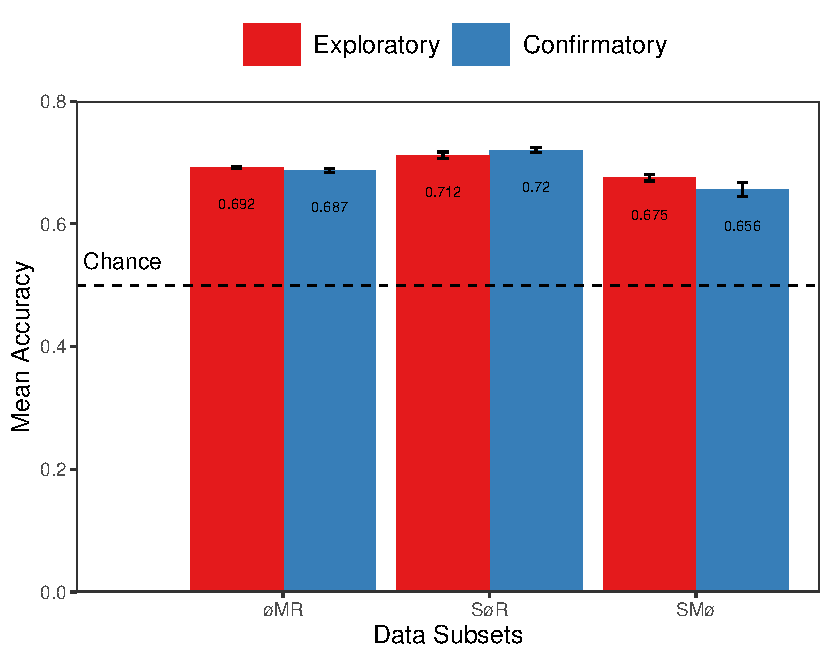
\includegraphics{supplementary_analysis/supp_subset_chance.pdf}
\caption{(\#fig:supp-chance)The graph represents the average accuracy
reported for each subset of the Exploratory and Confirmatory timeline
data. All of the data subsets were decoded at levels better than chance
(50\%). The error bars represent standard errors.}
\end{figure}

All of the data subsets analyzed in this supplementary analysis were
decoded with better than chance accuracy (see Figure
@ref(fig:supp-chance)). The same pattern of results was observed in both
the Exploratory and Confirmatory datasets. When the Memorize condition
was removed, classification accuracy improved (see Table
@ref(tab:supp-comparisons)). When the Rate condition was removed,
classification was the worst. When the Memorize condition was included,
the Memorize condition was more accurately predicted than the Search and
Rate conditions (see Figure @ref(fig:supp-conf-matrices)).

\begin{table}[!h]
    \centering
    \caption{Supplementary Subset Comparisons}
    \label{tab:supp-comparisons}
    \begin{tabular}{l c c c c}
         & \multicolumn{2}{c}{Exploratory} & \multicolumn{2}{c}{Confirmatory} \\
        \hline
        Comparison & \textit{t} & \multicolumn{1}{c|}{\textit{p}} & \textit{t} & \textit{p} \\
        \hline
        $\varnothing$MR vs. S$\varnothing$R & 3.248 & \multicolumn{1}{c|}{.008} & 3.094 & .012 \\
        $\varnothing$MR vs. SM$\varnothing$ & 2.875 & \multicolumn{1}{c|}{.021} & 2.923 & .018 \\
        S$\varnothing$R vs. SM$\varnothing$ & 6.123 & \multicolumn{1}{c|}{< .001} & 6.017 & < .001 \\
        \hline
    \end{tabular}
\end{table}

\begin{figure}
\centering
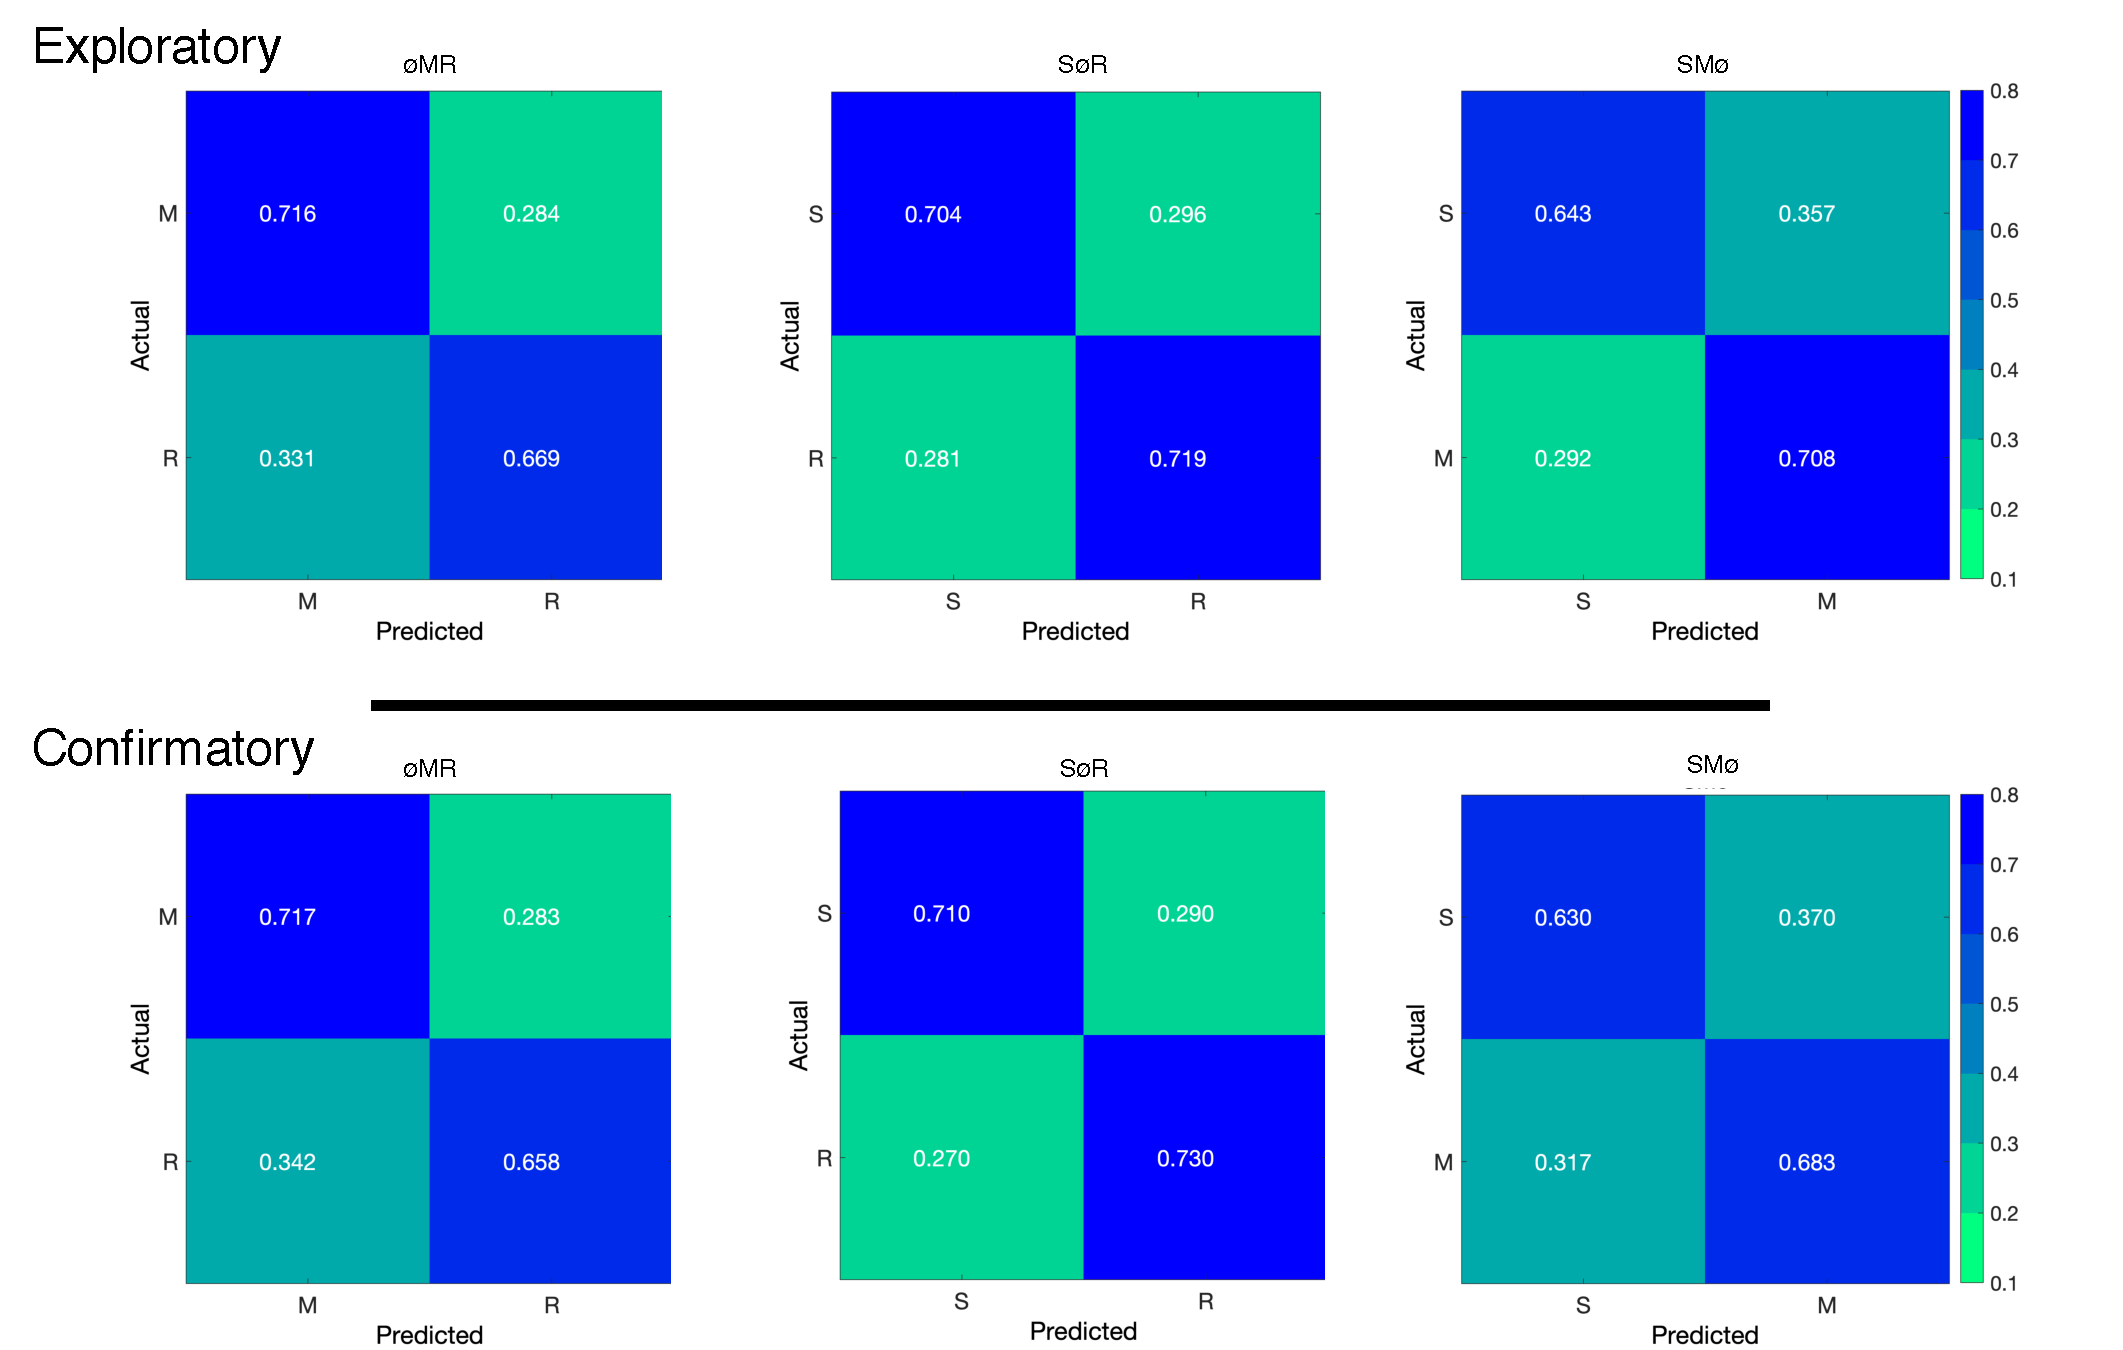
\includegraphics{supplementary_analysis/confusion_matrices/supp_conf_matrices.pdf}
\caption{(\#fig:supp-conf-matrices)The confusion matrices represent the
average classification accuracies for each condition of the timeline
data (S = Search, M = Memorize, R = Rate). The vertical axis of the
confusion matrices represents the actual condition for trial. The
horizontle axis of the confusion matrices represents the condition that
was predicted by the model.}
\end{figure}
\end{appendix}
